\section{Design} \label{sec:design}

\begin{figure}[t!] 
     \centering 
     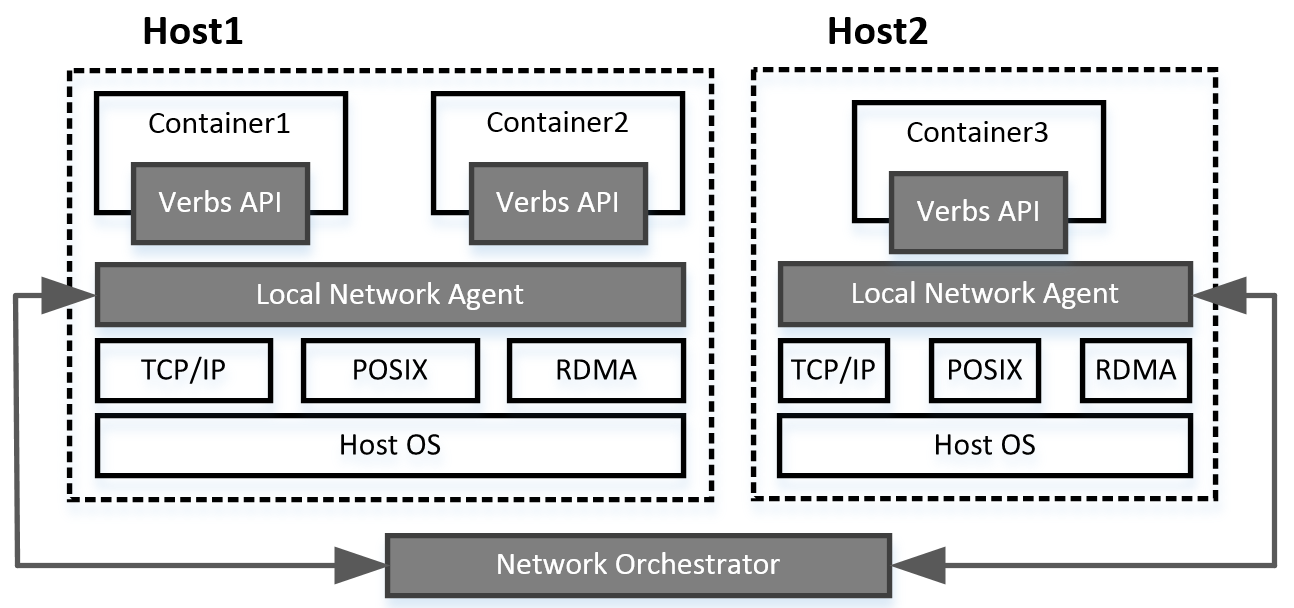
\includegraphics[width=3.2in]{figures/system-arch} 
    \caption{\label{fig:sysarch} The overall system architecture of~\sysname.} 
\end{figure} 

In this section, ...

\subsection{Overview}

Our goal is to design a completed network solution which can enable containers
to communicate with portability, isolation and high performance at the same time.
This solution has three main components: control-plane, data-plane and programing
abstraction. 

A flexible control-plane is a guarantee of portability and isolation. 
It should permit a container to register its own IP addresses in the network
from any host, and also should automatically configure and update the routing 
to each container. Different from existing overlay network solutions of 
containers, we also require the control-plane to be able to select 
data-plane protocols in real-time according to multiple factors, 
e.g. container locations, hardware capabilities, etc..

Data-plane should always promise the best network performance between 
containers. From measurements (Figure~\ref{XXX}), 
we see that shared-memory has the highest
bandwidth, lowest latency, smallest NIC load and modest CPU load. 
Therefore, shared-memory is favorable to be used as the data-plane 
mechanism between two containers on the same host. 
The data-plane for inter-host communication
depends on the hardware capability. RDMA is preferred to TCP/IP if the NICs
on the hosts have the support.

A network programming abstraction defines how communication is performed.
People have designed multiple network abstractions used in different scenarios.
For example, the most popular network abstraction for TCP/IP is Socket~\cite{?},
Verbs~\cite{?} is widely accepted for RDMA, and MPI~\cite{?} is a standard for
message-passing in distributed memory and parallel computers. We require that
the network programming abstraction must at least have two
properties. First, it facilitates containers to access the network and 
transparently utilize the data-plane mechanisms, and second, it is general 
enough to support existing programming interfaces on top of it for backward 
compatibility.

The design of~\sysname fully considers the requirements from all these three
components.

\subsection{The architecture of FreeFlow}

Figure~\ref{fig:sysarch} shows the architecture and design choices on each 
components of~\sysname.

\para{Centralized control-plane:}

\para{RDMA/Shared-Memory based Data-plane:}

\para{Verbs based programming abstraction:}

